% chapters/07_compliance.tex
\chapter{合规、来源与 AI 声明}

\section{概述}

根据全国操作系统设计赛的技术方案要求，参赛队必须对作品中复制的代码和文档来源进行明确说明，并严格遵守相关开源协议。同时，使用 AI 工具的参赛队需在设计实现文档中声明 AI 工具的名称、使用场景及交互记录。

本章独立成章，全面披露本项目的代码来源、开源协议合规性、借鉴基础与增量贡献，以及 AI 工具的使用情况。

\section{代码与文档来源及开源协议说明}

\subsection{引用的开源代码}

本项目在开发过程中参考或引用了以下开源代码和依赖库：

\begin{table}[H]
    \centering
    \caption{引用的开源代码与依赖库}
    \label{tab:open_source_refs}
    \begin{tabular}{p{0.20\textwidth}p{0.35\textwidth}p{0.35\textwidth}}
        \toprule
        \textbf{名称} & \textbf{来源/URL} & \textbf{使用目的} \\
        \midrule
        星绽操作系统（Asterinas） & https://github.com/asterinas/asterinas & 基础操作系统框架和 OSTD 接口 \\
        aes crate & https://crates.io/crates/aes & AES 加密算法实现 \\
        xts-mode crate & https://crates.io/crates/xts-mode & XTS 加密模式实现 \\
        \bottomrule
    \end{tabular}
\end{table}

\subsection{开源协议合规性声明}

本项目严格遵守以下开源协议要求：

\begin{itemize}
    \item \textbf{项目源代码}：遵循 Apache-2.0 开源协议。
    \item \textbf{技术文档与答辩材料}：遵循 CC-BY-SA 4.0 开源协议。
    \item \textbf{第三方依赖}：所有引用的 Rust crate 均遵循其各自的开源协议（主要为 MIT 或 Apache-2.0），与本项目的协议兼容。
\end{itemize}

\section{借鉴基础版本与增量贡献说明}

\subsection{借鉴基础}

本项目的设计与实现深受以下基础项目和技术的启发：

\begin{itemize}
    \item \textbf{Linux 内核 Device Mapper 框架}：dm-crypt 和 dm-verity 的功能逻辑和表格式规范参考了 Linux 内核的成熟设计。
    \item \textbf{星绽操作系统 Framekernel 架构}：基于星绽的 OSTD 框架和 BlockDevice 抽象进行适配和集成。
    \item \textbf{Rust 生态的密码学库}：借鉴了 aes 和 xts-mode crate 的接口设计和安全实践。
\end{itemize}

\subsection{本队增量贡献}

在借鉴上述基础版本的基础上，本项目的核心增量贡献包括：

\begin{itemize}
    \item \textbf{统一的 BlockDevice Trait 抽象}：设计了与平台无关的块设备抽象层，使得同一套核心代码能够同时运行于用户态和星绽内核态。
    \item \textbf{纯 Rust 实现的 SHA-256}：独立实现了 FIPS 180-4 标准的 SHA-256 哈希算法。
    \item \textbf{星绽内核完整集成}：通过可审计 Git 补丁序列将 dm-crypt 和 dm-verity 完整集成到星绽内核中。
    \item \textbf{内核启动自检机制}：实现了基于 ext2 超级块魔数的启动时自检。
    \item \textbf{五阶段渐进式保护路径}：设计并实现了从 Plain 到 Combined 的渐进式安全保护路径。
    \item \textbf{性能优化}：实现了认证后哈希块缓存、完成 BIO 数据复用、有界临时缓冲池和 AES-NI 硬件加速，并为新优化保留独立 A/B 开关。
\end{itemize}

\section{AI 工具使用声明}

本项目在开发过程中，严格遵守比赛关于"允许参赛学生合理使用 AI 工具"的规定。

\subsection{使用的 AI 工具及大模型}

\begin{table}[H]
    \centering
    \caption{AI 工具使用详情}
    \label{tab:ai_tools}
    \begin{tabular}{p{0.18\textwidth}p{0.18\textwidth}p{0.55\textwidth}}
        \toprule
        \textbf{工具名称} & \textbf{相关大模型} & \textbf{具体使用场景与辅助内容} \\
        \midrule
        OpenAI Codex & GPT-5 & 1. 阅读和梳理星绽框架、dm-crypt、dm-verity 相关底层代码；\\
         & & 2. 辅助分析 BIO 数据路径与编译错误；\\
         & & 3. 生成或修改部分 Rust、Shell 测试和构建脚本；\\
         & & 4. 协助整理参赛文档表述。 \\
        \midrule
        通义千问（Qwen） & Qwen-Max & 技术文档的深度润色，确保中英文专业术语的准确性与一致性。 \\
        \midrule
        豆包（Doubao） & 豆包大模型 & 答辩表述的逻辑优化，整理技术答辩常见问题及应对策略。 \\
        \bottomrule
    \end{tabular}
\end{table}

\subsection{AI 交互记录}

以下是开发过程中与 AI 工具的关键交互截图，证明 AI 仅作为辅助工具，开发逻辑由团队主导。

\subsubsection{OpenAI Codex 交互记录（GPT-5）}

\begin{figure}[H]
    \centering
    \begin{subfigure}[b]{0.45\textwidth}
        \centering
        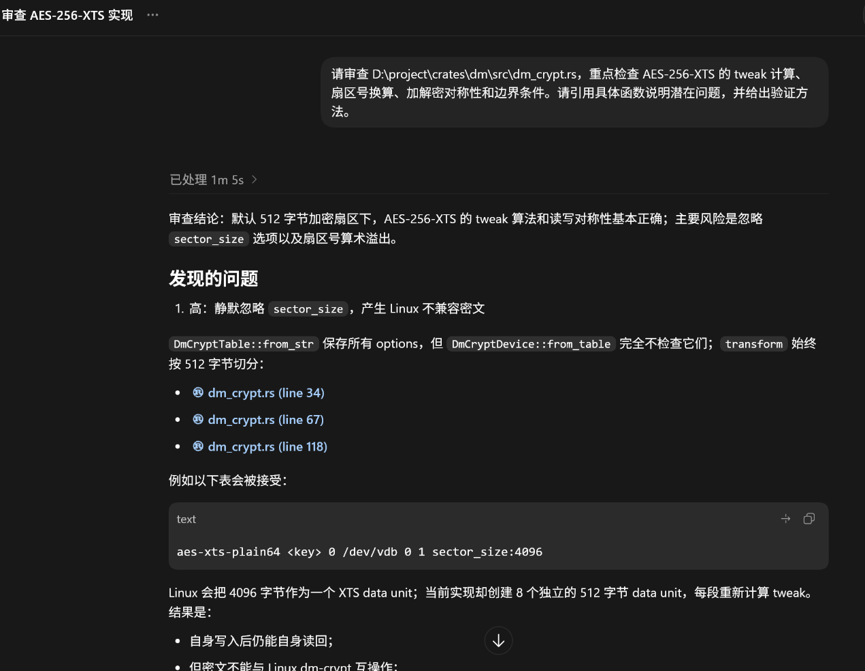
\includegraphics[width=\textwidth]{figures/codex_ai_1.png}
        \caption{代码分析与框架理解}
        \label{fig:codex_1}
    \end{subfigure}
    \hfill
    \begin{subfigure}[b]{0.45\textwidth}
        \centering
        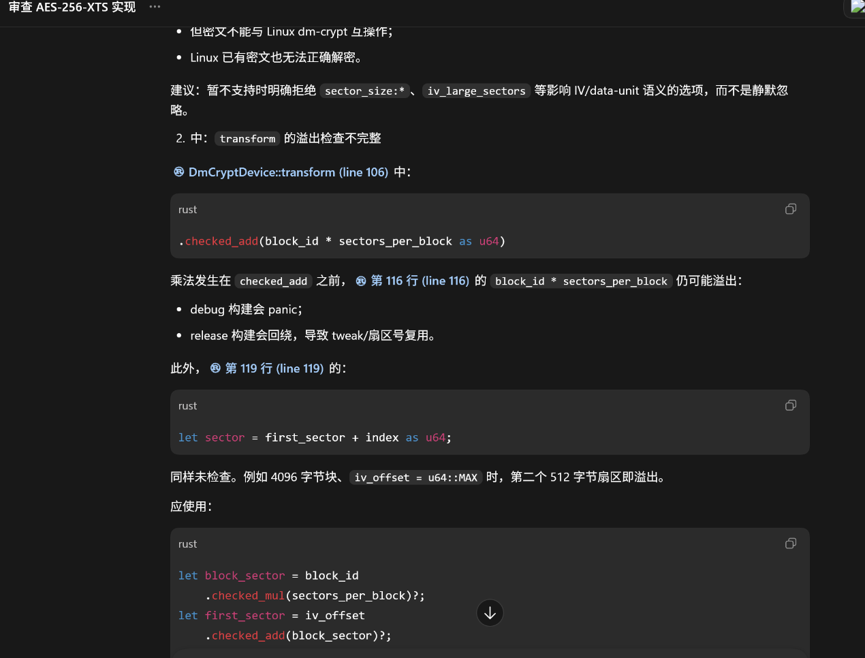
\includegraphics[width=\textwidth]{figures/codex_ai_2.png}
        \caption{BIO 路径辅助分析}
        \label{fig:codex_2}
    \end{subfigure}
    \caption{OpenAI Codex 交互记录（1/4）}
    \label{fig:codex_group1}
\end{figure}

\begin{figure}[H]
    \centering
    \begin{subfigure}[b]{0.45\textwidth}
        \centering
        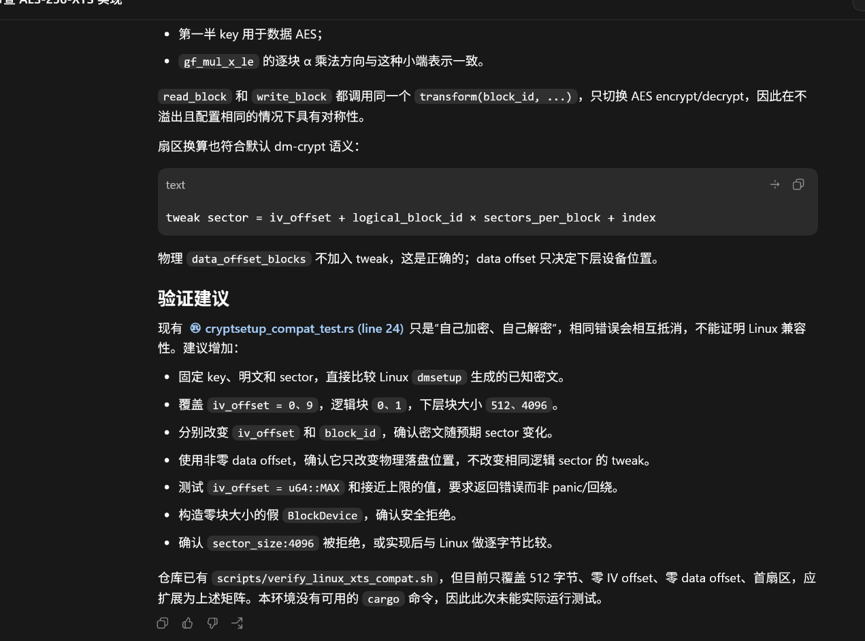
\includegraphics[width=\textwidth]{figures/codex_ai_3.png}
        \caption{Rust 测试脚本生成}
        \label{fig:codex_3}
    \end{subfigure}
    \hfill
    \begin{subfigure}[b]{0.45\textwidth}
        \centering
        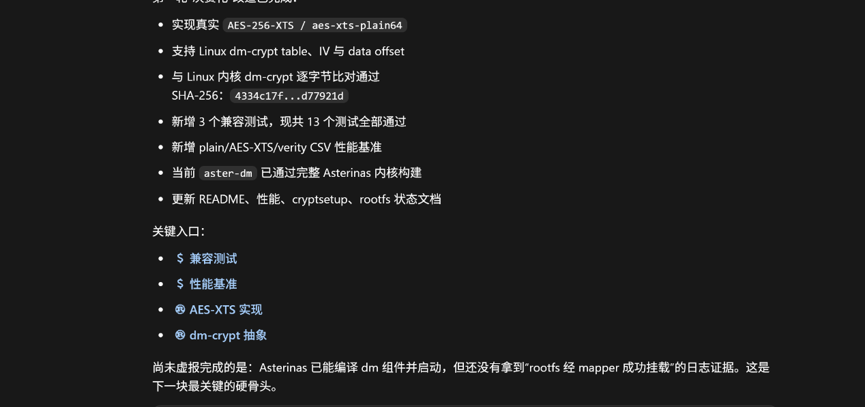
\includegraphics[width=\textwidth]{figures/codex_ai_4.png}
        \caption{Shell 构建脚本辅助}
        \label{fig:codex_4}
    \end{subfigure}
    \caption{OpenAI Codex 交互记录（2/4）}
    \label{fig:codex_group2}
\end{figure}

\begin{figure}[H]
    \centering
    \begin{subfigure}[b]{0.45\textwidth}
        \centering
        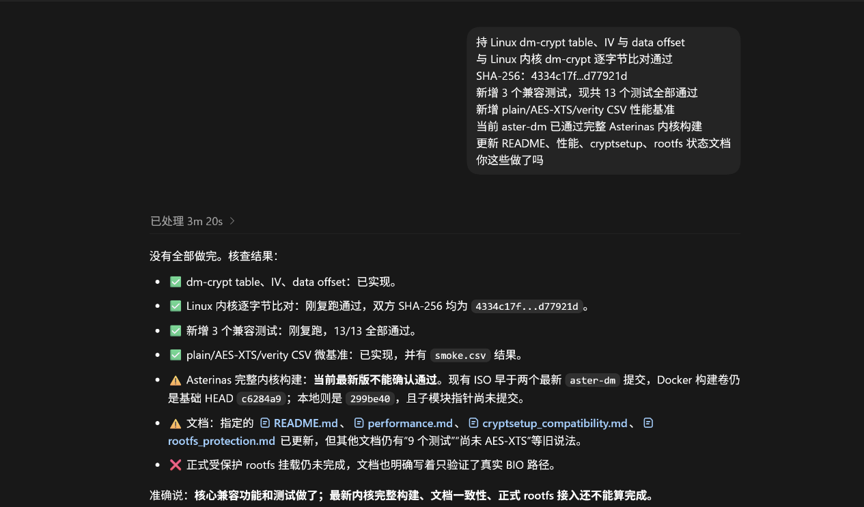
\includegraphics[width=\textwidth]{figures/codex_ai_5.png}
        \caption{QEMU 日志解读}
        \label{fig:codex_5}
    \end{subfigure}
    \hfill
    \begin{subfigure}[b]{0.45\textwidth}
        \centering
        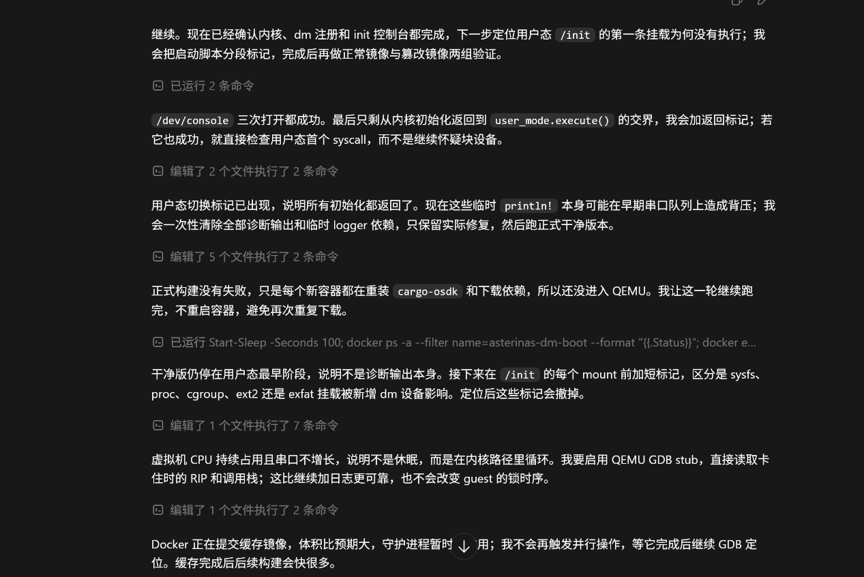
\includegraphics[width=\textwidth]{figures/codex_ai_6.png}
        \caption{编译错误调试}
        \label{fig:codex_6}
    \end{subfigure}
    \caption{OpenAI Codex 交互记录（3/4）}
    \label{fig:codex_group3}
\end{figure}

\begin{figure}[H]
    \centering
    \begin{subfigure}[b]{0.45\textwidth}
        \centering
        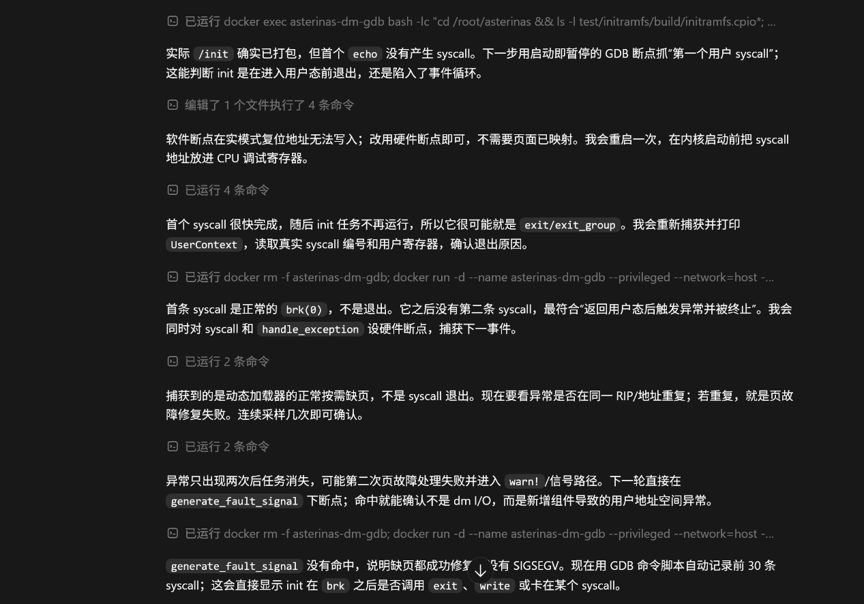
\includegraphics[width=\textwidth]{figures/codex_ai_7.png}
        \caption{内核 panic 追踪}
        \label{fig:codex_7}
    \end{subfigure}
    \hfill
    \begin{subfigure}[b]{0.45\textwidth}
        \centering
        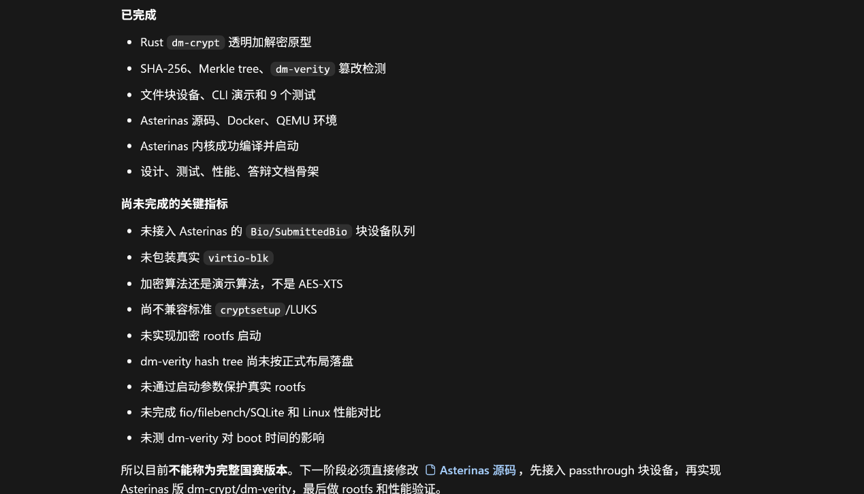
\includegraphics[width=\textwidth]{figures/codex_ai_8.png}
        \caption{文档表述整理}
        \label{fig:codex_8}
    \end{subfigure}
    \caption{OpenAI Codex 交互记录（4/4）}
    \label{fig:codex_group4}
\end{figure}

\subsubsection{通义千问（Qwen）交互记录}

\begin{figure}[H]
    \centering
    \begin{subfigure}[b]{0.45\textwidth}
        \centering
        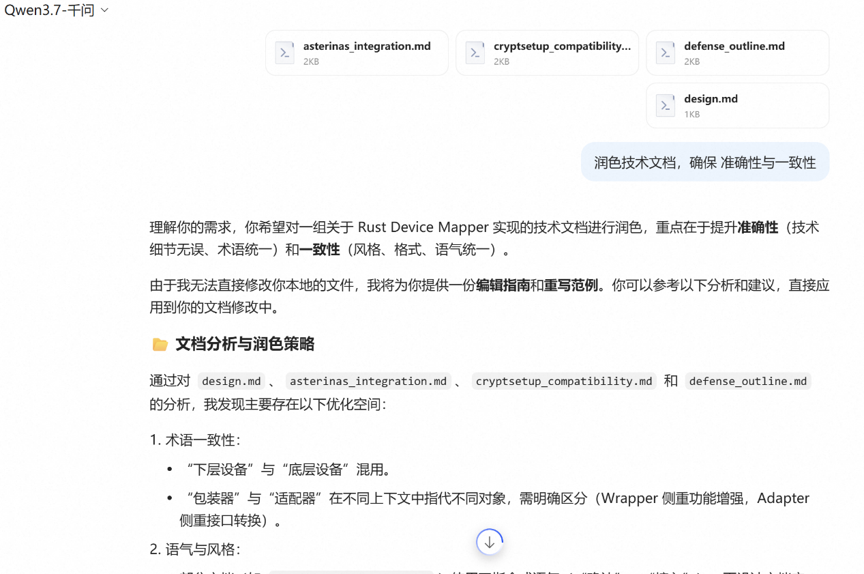
\includegraphics[width=\textwidth]{figures/qwen_ai_1.png}
        \caption{技术文档润色}
        \label{fig:qwen_1}
    \end{subfigure}
    \hfill
    \begin{subfigure}[b]{0.45\textwidth}
        \centering
        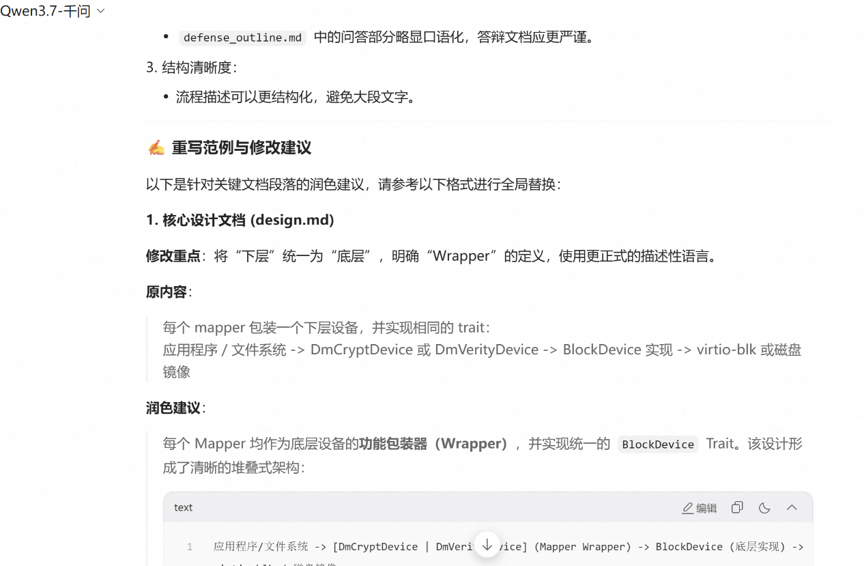
\includegraphics[width=\textwidth]{figures/qwen_ai_2.png}
        \caption{专业术语校对}
        \label{fig:qwen_2}
    \end{subfigure}
    \caption{通义千问（Qwen）交互记录}
    \label{fig:qwen_group}
\end{figure}

\subsubsection{豆包（Doubao）交互记录}

\begin{figure}[H]
    \centering
    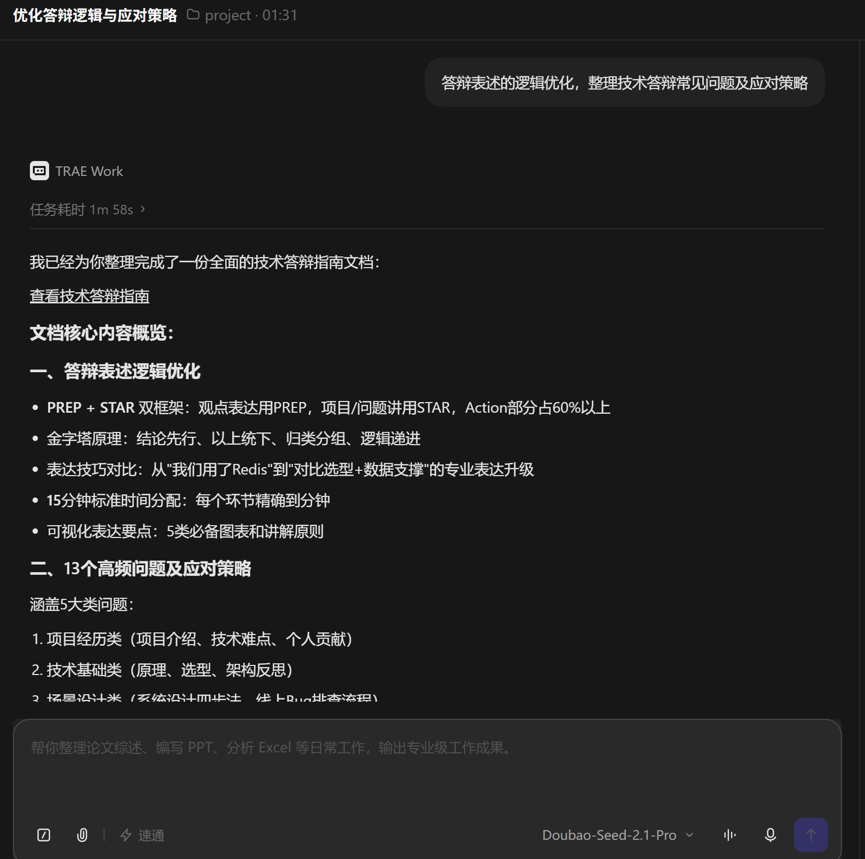
\includegraphics[width=0.8\textwidth]{figures/doubao_ai_1.png}
    \caption{豆包（Doubao）答辩表述优化与 FAQ 整理}
    \label{fig:doubao_1}
\end{figure}

\subsection{验证机制与责任声明}

为确保代码与文档的质量及原创性，项目组采取了以下严格措施：

\begin{enumerate}
    \item \textbf{人工审查}：所有 AI 生成的代码片段和文档内容，均经过团队成员的人工 Peer Review。
    \item \textbf{交叉验证}：代码正确性通过严格的单元测试、与 Linux dm-crypt 的逐字节对照、星绽内核构建及 QEMU 端到端运行进行了多重验证。
    \item \textbf{责任承担}：最终的技术方案、代码取舍、架构决策和提交材料均由参赛团队全权负责。
\end{enumerate}

\section{Git 提交与开发迭代记录}

\subsection{提交概览}

\begin{table}[H]
    \centering
    \caption{Git 提交记录概览}
    \label{tab:git_commits}
    \begin{tabular}{p{0.08\textwidth}p{0.12\textwidth}p{0.18\textwidth}p{0.32\textwidth}p{0.20\textwidth}}
        \toprule
        \textbf{序号} & \textbf{提交时间} & \textbf{Commit Hash} & \textbf{提交说明} & \textbf{变更统计} \\
        \midrule
        1 & 06-23 14:15 & 6bb9bc9 & 初始提交，仅源码 & 44 文件，+2500 行 \\
        2 & 06-23 22:36 & 40a5217 & 增加 Linux 兼容的 Device Mapper 实现 & 18 文件，+1923/-61 行 \\
        3 & 06-23 22:58 & c72462b & 验证 Asterinas dm BIO 路径 & 6 文件，+280/-12 行 \\
        4 & 06-24 01:33 & 2f8a671 & 接入受保护根文件系统 & 12 文件，+186/-25 行 \\
        5 & 06-24 01:42 & a0dbb0f & 补充国产 AI 工具使用说明 & 1 文件，+4 行 \\
        6 & 06-24 01:48 & 84970aa & 修改文档（文档中文化） & 6 文件，+118/-113 行 \\
        \bottomrule
    \end{tabular}
\end{table}

\begin{figure}[H]
    \centering
    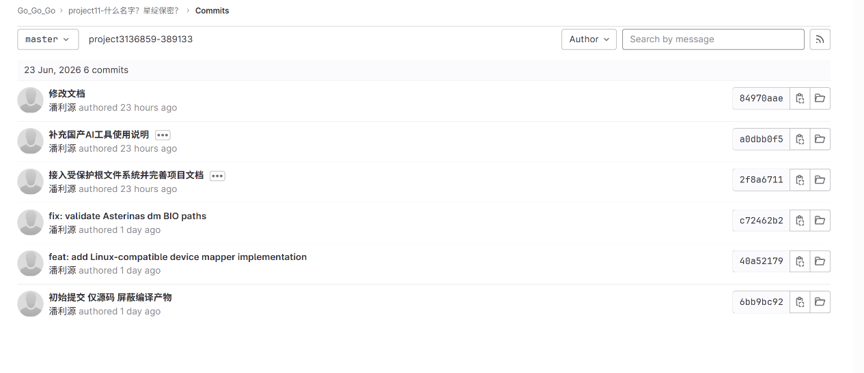
\includegraphics[width=0.9\textwidth]{figures/git_commit_history.png}
    \caption{GitLab 仓库提交历史截图}
    \label{fig:git_history}
\end{figure}

\subsection{关键迭代节点说明}

\begin{enumerate}
    \item \textbf{基础架构与核心逻辑}：完成了 BlockDevice trait 的抽象，实现了纯 Rust 的 AES-256-XTS 加密与 SHA-256 默克尔树校验。
    \item \textbf{内核集成与 BIO 路径打通}：将用户态逻辑移植至星绽内核，成功实现了基于 pivot\_root 的受保护根文件系统切换。
    \item \textbf{文档与合规性完善}：全面梳理技术文档，完成中文化翻译，并补充 AI 工具使用声明。
\end{enumerate}

\section{小结}

本章严格按照全国操作系统设计赛的技术方案要求，全面披露了本项目的代码来源、开源协议合规性、借鉴基础与增量贡献、AI 工具使用声明以及 Git 提交与开发迭代记录。所有引用和借鉴的内容均已明确标注来源，所有 AI 辅助生成的内容均经过人工审查和验证。
